\documentclass[12pt, letterpaper]{article}

\title{Final Project Report: SMASH}
\author{Nathan Roach, Patricia Walchessen, Charlie Wang, and Yue Zhang}
\date{December 8, 2017}

\usepackage[utf8]{inputenc}
\usepackage{blindtext}
\usepackage{cite}
\usepackage{color}
\usepackage{comment}
\usepackage{csquotes}
\usepackage{graphicx}
\usepackage[numbers]{natbib}
\usepackage{wrapfig}


\setlength{\parindent}{4em}
\setlength{\parskip}{1em}

\begin{document}

\maketitle

\begin{abstract}
	[1 paragraph] \color{red} TO DO \color{black} Final Project Abstract
\end{abstract}


\section{Introduction}
An intriguing and common problem that arises in computation is efficiently comparing the similiarities between high-dimensional data. The problem reaches into the far corners of computation, including machine learning and kernels. In bioinformatics, the problem takes the form of determining the similarity between both close and disparate long genomic sequences. Solving the challenge of comparing long genomic sequences would aid in evaluating evolutionary relationships, determining the organismal source of sequencing data, and comparing metagenomic data. \\ \\
One class of algorithms that could solve this problem is Locality-Sensitive Hashing (LSH) algorithms. LSH algorithms reduce data dimensionality and bin inputs such that similar data sets are grouped together with high probability. They solve the problem of approximate or exact Near Neighbor Search. In recent years LSH algorithms have offered solutions to problems such as: near-duplicate detection, genome-wide association, and both image and audio similarity identification. There are two prevalent LSH algorithms: MinHash and SimHash. \\ \\
MinHash computes the differences between two genomic sequences through the estimation of a Jaccard Index, a ratio of the  shared identity between the sets. SimHash, on the other hand, estimates the cosine similarity by weighting of the frequency of bits, compiling them into vectors and evaluating similarity by the distance between the vectors.

\section{Prior Work}
\begin{verbatim*}
[1 page] \color{red} TO DO \color{black} In 2016, Ondov et al. used MinHash to analyze the resemblance between genomes and metagenomes\cite{MinHash}. They altered the MinHash algorithm to include pairwise mutation distance, or Mash distance, which estimates the rate of sequence mutation under a simple evolutionary model. Their modifications allowed Mash to efficiently cluster and search of massive sequence collections. Mash, as they call their implementation, has two main components: \testit{sketch} and \testit{dist}. The \testit{sketch} funciton creates MinHash sketches from a sequence or a collection of sequences. \testit{Dist} compares two sketches and returns an estimate of the Jaccard index (ratio of the shared identity between sets), a P value, and the Mash distance.\ref{fig:MinHashDescription} Two important parameters within Mash are sketch size and k-mer size. A larger sketch size improves accuracy of the Mash estimates, particularly for divergent genomes, but increases the space and time required for computing distances. The determination of k-mer size alters sensitivity and specificity. Smaller values of k-mer size are more sensitive for divergent genomes, but lose specificity for large genomes due to k-mer collisions. Larger values of k-mer size lose sensitivity. Thus, chosing the smallest k-mer size that reduces chance collisions is important and the k-mer size will change depending on the divergence of the genomes. To maximize sensitivity and specificity, Mash uses a default k-mer size of 21 and a sketch size of 1,000. According to preliminary research by Ondov et al., Mash can be used to cluster whole genomes, identify the genome in real-time  from assemblies or reads, and cluster massive metagenomic databases.\\ \\
\end{verbatim*}


% Mash description Figure
\begin{wrapfigure}{c}{0.25\textwidth}
    \centering
    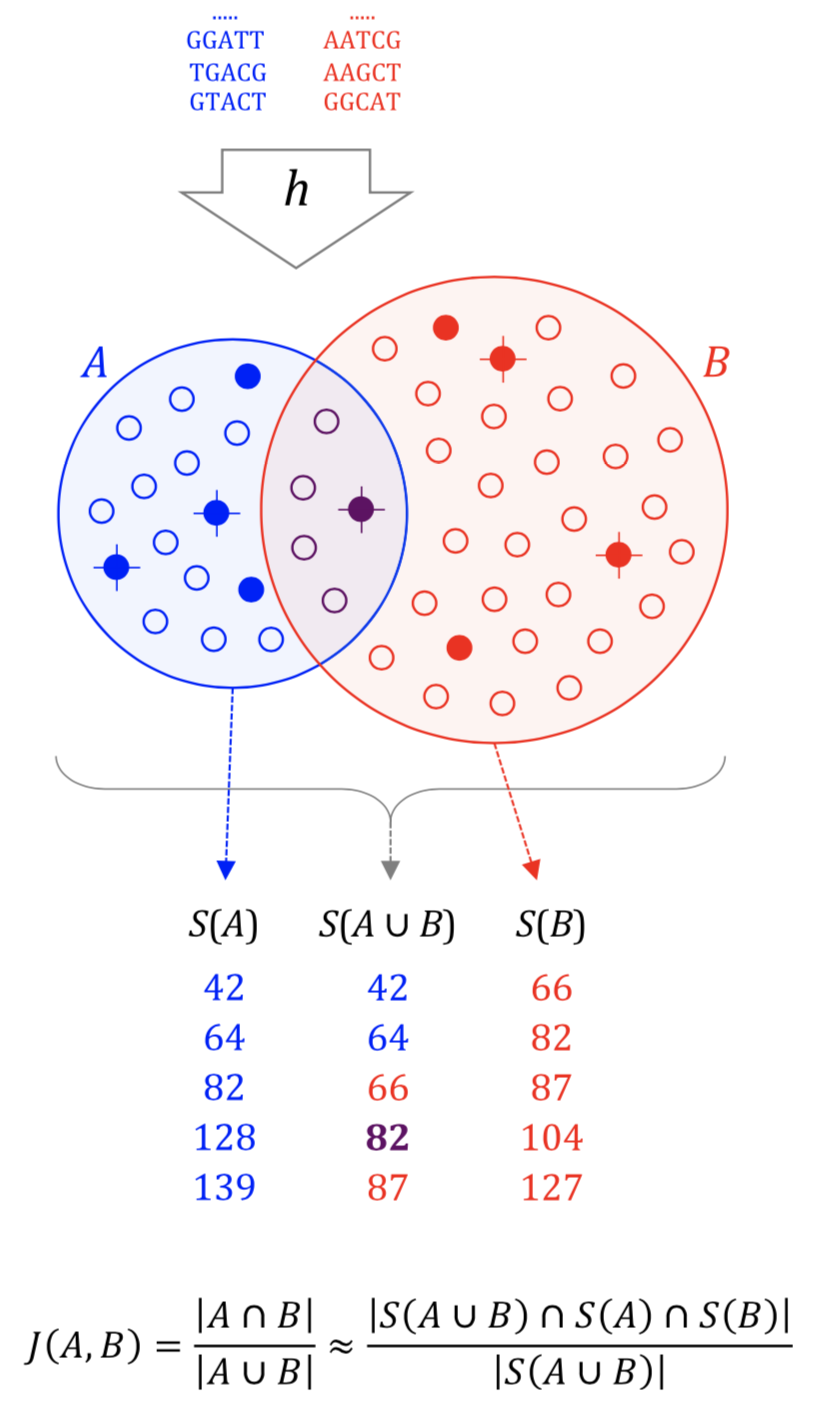
\includegraphics[width=0.25\textwidth]{Mash_description.png}
    \caption{Description of MinHash: First, the sequences divided into their constituent k-mers. Each k-mer is then passed through a hash function to obtain a 32- or 64-bit hash. The Jaccard index is ratio of shared hashes between A and B over all distinct hashes in A and B. The Jaccard Index can be approximated by considering a smaller subset of A and B. MinHash sketches S(A) and S(B) of size 5 are shown for A and B, comprising the five smallest hash values. The Jaccard Index is determined by dividing the similarity between S(A) and S(B) by the distinct values in S(A) and S(B)}
\label{fig:MinHashDescription}
\end{wrapfigure}

Mash has been used to cluster all of the NCBI RefSeq Release 70, totaling 54,118 organisms and 618 Gbp of genomic sequence. The resulting sketches yielded a compression factor of more than 7000-fold versus the uncompressed FASTA (93 MB vs. 674 GB) and only took 33 CPU hours. Additionally, adding a genome to the database took approximately 0.9 CPU seconds per 5 MB genome. However, fast and space-efficient only works if the results are valid. A comparison of Mash distance and ANI, a  measure of genetic similarity, among a subset of 500 E. coli genomes, found Mash distances correlate well with ANI. For a sketch size of 1,000 and k-mer size of 21, Mash approximates 1 - ANI with a root-mean-square error of 0.00274. Thus, Mash enables scalable, whole-genome clustering. 

With a pre-computed sketch database, Mash is able to identify isolated genomes from both assemblies within a few seconds and identify the Lowest Common Ancestor (LCA) from raw sequencing reads within a couple of minutes. Additional work is needed until Mash can be used to discern genome identity from raw sequencing reads, possibly by filtering out low frequency k-mers or increasing the sketch size.

Mash can also cluster metagenomic datasets in a fraction of the time other metagenomic comparison tools use. DSM, which uses an exact Jaccard Index, and COMMET, which attempts to identify a set of similar reads between two samples using Bloom filters, are both metagenomic comparison tools commonly used today. In a comparison between COMMET and Mash on a pool of Global Ocean Survey (GOS) data, Mash was over ten times faster than COMMET and correctly identified clusters from the original GOS study. Thus, Mash provided a time efficient way to analyze and cluster large-scale metagenomic data.

Mash enables the comparison and clustering of whole genomes and metagenomes on a massive scale. However, after additional research, we saw no reference of using any other LSH to hash and compare genomic sequences, so we pursued a research project on a competing LSH algorithm: SimHash. Previous studies suggest SimHash can be used for the same purpose as MinHash in analyzing resemblance. 

\section{Research Methods and Software}


\subsection{Exploration with MinHash}
We explored the algorithm and libraries of MinHash to better understand the properties behind MinHash, better understand how MinHash performs and works, and to confirm that we are able to achieve the results of the MASH paper. To accomplish this, we used a Python implementation of Mash called SourMash\cite{GitHub-Sourmash}, which was developed by Titus Brown and Luiz Irber from UC Davis and is available open-source. The data that we ran the MinHash library on was 300+ E. coli genomes, which were compared between each other. We achieved and determined a minimum distance of 0.378. \color{red} TO DO \color{black} \ref{fig:All Ecoli} The E. coli genomes were downloaded from the RefSeq database and a full list is available in the appendix.


\subsection{Exploration with SimHash}
\subsubsection{Dataset}
The data that we tested on included 300+ E. coli genomes as well as multiple different yeast genomes. For the purpose of the discussion in this section, we will talk about the methods developed based on empirical testing on a dataset consisting of 1 E. coli genome and 2 yeast genomes named S. cerevisiae, S. pombe. Additional discussion of the complete dataset will be presented in the Results section.

\subsubsection{Method}
To fully explore the application of SimHash in the genomics field, we commenced with surveying the existing SimHash literature and implementations. Next, we looked for existing SimHash libraries, many of which were designed for analyzing websites are texts of English words, and compiled the most reputable ones. From there, we selected two based on their reputation and fork numbers for us to base our code on and to adapt into the genomic field to explore SimHash more extensively. The first is Python-based (https://github.com/leonsim/simhash) and the second is Go-based (https://github.com/mfonda/simhash). \color{red} Cite properly \color{black}

\subsubsection{Python-based SimHash}
Upon surveying the existing code in the Python-based SimHash, we found that there were some hard-coded values in the library, such as k-mer or shingles sizes of 4. We thus took account of hard-coded values, and then created our own SimHash class based on the Python-based SimHash. The goal with our SimHash class is to enable it to fundamentally accept genomic data and build the shingles based on genomic data, not say English words. One thing to note when we explored the Python-based SimHash was that it relied on using MD5 to hash the keys, and then performed the operations of SimHash and the hamming distance on the MD5 hashes. The hashes were also of 32 bit. In all, we coded a more flexible Python-based SimHash library for running our tests of SimHash on genomic data.

\subsubsection{Go-based SimHash}
Our design and coding of the Go-based SimHash was similar to the Python-based SimHash. By basing our code on the Go library, we made a fundamental modification to accept genomic data. A special particularity with the unmodified Go-based SimHash library is that though the library has the method for making shingles of words, it does not appear to be used. Also, the unmodified Go-based SimHash library very much assumes that the input is string of English words that could or could not be encoded in Unicode. Thus, we made fundamental modifications to the feature construction in the Go-based SimHash library to accept genomic data. Some of the modifications included building the features based on whether it is a substring of lowercase bases or uppercase bases, or building the features based on a k-mer size of say 15. We continued with the use of 64 bit hashes in Go.


\subsubsection{Evolution of our Research}
With both our Python-based SimHash and Go-based SimHash code, we fed in the genomic data to test how the core SimHash algorithm performs. Recall that the genomic data consisted of one strain of E. coli, which is about 4.5 million bases, while both of the yeast strands are about 12 million bases each. After running the SimHash algorithm in each respective language and observing the output of the distance between the genomic data, we found that the results were lackluster. \\ \\
While say between one of the yeast strands and the E. coli, the SimHash algorithm was able to distinguish that they were quite different, the SimHash algorithm outputted that the difference between the other yeast strand and E. coli vs. the difference between both of the yeast strands was about equivalent. Fundamentally, just from the fact that E. coli is a much shorter genome, the result showed that SimHash was losing some sort of resolution. \\ \\
We first thought that it might be due to how the Python-based SimHash was using the MD5 hash and was implementing SimHash that influenced the results. However, by bringing in the Go-based SimHash which does not use a MD5 hash but the raw bit values and computes the SimHash fingerprint based on a bit by bit operation with weighting, which is a bit different than the Python-based SimHash, the fact that both were returning similarly lackluster results showed that the implementation of SimHash is not likely the factor.  \\ \\
We next explored whether it is because of how we are inputting the genomic data. We explored different k-mer sizes and also decided to normalize the data by converting say all the bases to lowercase letters. However, even attempts at standardizing the genomic data or exploration of different shingling sizes did not alter the lackluster results outputted from SimHash. Thus, we concluded that it is likely due to how the SimHash algorithm is designed. \\ \\
We explored the literature online, and discovered that SimHash was primarily designed for finding small discrepancies between websites. Thus, the design principle of SimHash was to have a good high resolution of small amount of changes. Thus, it can be implied that SimHash is unable to accurately handle too big of changes or hamming distances. With say a hamming distance of over 20, SimHash would start losing resolution of the distance between the hashes. Thus, we needed to find a way to make up for the loss of resolution.


\subsection{SMASH}
Thus came the development of original research based on what we learned and observed from MinHash and SimHash. Seeing how the existing SimHash algorithm was losing resolution when the Hamming distance was too great, we went back to the drawing board and examined each part of the SimHash algorithm closely. From the examination and with additional brainstorming, we came up with SMASH, which is designed to primarily address the shortcoming of resolution loss with SimHash.

\subsubsection{Design}
One of the major loss of resolution with SimHash was with the following: when a E. Coli genome with some 4.5 million bases is compared to one of the yeast genomes with 12 million bases, SimHash outputs that it is about the same hamming distance apart as another comparison, which is instead between to two yeast genomes and which both of which have about 12 million bases. Thus, we sought to address the loss of frequency in the resolution.  \\ \\
First, we observed that the basic property of the LSHs were the consensus to find a way to build a feature structure out of the dataset. In our case, we decided to build our feature structure based on frequency. The way this is handled is that for each of the genome file that is inputted, we parse it such that it becomes one complete contiguous string. Next, we chop it up into the respective k-mers. An important thing to note is that the size of the k-mer needs to be specified beforehand, and thus we test for the optimal k-mer size and describe it in the Results section. The frequency is based on how frequently the k-mers show up in the respective genome files. \\ \\
Based on the order of the feature structure, we then construct vectors consisting of the frequency of the k-mers. This is then fed into the cosine similarity function, which is used in SimHash, to compute the cosine similarity. Notice that a fundamental difference between SimHash and SMASH is that while SimHash focuses on computing a weighting of frequency of bits, SMASH is instead focusing on computing a weighting of frequency of k-mers. For a finer look into what SMASH does, the pseudocode for the algorithm is accompanied in the next section.

\subsubsection{Algorithm}
\begin{verbatim}
file1, file2 = input 2 genome files 
k = k-mer size

for each file:
    parse and format into one contiguous string

for each file:
    file1_kmers, file2_kmers = divide up file into k-mers

file1_count = dict()
file2_count = dict()

for each kmer in file1_kmers:
    file1_count[kmer] += 1

for each kmer in file2_kmers:
    file2_count[kmer] += 2

for subset of observed k-mers in file_1:
    vector1 = vector of kmer counts from file1_count

for subset of observed k-mers in file_2:
    vector2 = vector of kmer counts from file2_count

similarity_distance = 1 - cosine(vector1, vector2)
\end{verbatim}




\section{Contributions of Each Member}
[1 paragraph] \color{red} TO DO \color{black}

\section{Results}
[1.5 pages] \color{red} TO DO \color{black} Insert results of different k-mer sizes and of different genomic sequences.

\section{Conclusions}
[0.5 pages] \color{red} TO DO \color{black} There are more ways to judge similarity between two genomic sequences than just hashing the entirety of each of the genome and comparing how close in relation both are.



% ---------------------------------------------------------------------------------------------------------------------------
% Bibliography
% ---------------------------------------------------------------------------------------------------------------------------
\begin{thebibliography}{9}

\bibitem{GitHub-SourMash} 
  C. Titus Brown and Luiz C. Irber, Jr.
  \textit{SourMash}.
  GitHub repository, https://github.com/dib-lab/sourmash, 2016.
  
\bibitem{simhash} 
  Caitlin Sadowski and Greg Levin.
  \textit{SimHash: Hash-based Similarity Detection}.
  http://citeseerx.ist.psu.edu/viewdoc/download?doi=10.1.1.473.7179\&rep\\=rep1\&type=pdf, 
  2007.

\bibitem{SimvsMin} 
  Anshumali Shrivastava and Ping Li.
  \textit{In Defense of MinHash Over SimHash}.
  Journal of Machine Learning, 33, 2014.

\bibitem{MinHash} 
  Brian D. Ondov, Todd J. Treangen, Páll Melsted, Adam B. Mallonee, Nicholas H. Bergman, Sergey Koren and Adam M. Phillippy.
  \textit{Mash: fast genome and metagenome distance estimation using MinHash}.
  Genome Biology, 17:132, 2016.

\end{thebibliography}

\clearpage
% ---------------------------------------------------------------------------------------------------------------------------
% Appendix
% ---------------------------------------------------------------------------------------------------------------------------
\appendix

\section{E. Coli Genomes}
\begin{verbatim*}
GCF_000005845.2_ASM584v2_genomic.fna.gz
GCF_000007445.1_ASM744v1_genomic.fna.gz
GCF_000008865.1_ASM886v1_genomic.fna.gz
GCF_000009565.1_ASM956v1_genomic.fna.gz
GCF_000010245.2_ASM1024v1_genomic.fna.gz
GCF_000010385.1_ASM1038v1_genomic.fna.gz
GCF_000010485.1_ASM1048v1_genomic.fna.gz
GCF_000010745.1_ASM1074v1_genomic.fna.gz
GCF_000010765.1_ASM1076v1_genomic.fna.gz
GCF_000013265.1_ASM1326v1_genomic.fna.gz
GCF_000013305.1_ASM1330v1_genomic.fna.gz
GCF_000014845.1_ASM1484v1_genomic.fna.gz
GCF_000017745.1_ASM1774v1_genomic.fna.gz
GCF_000017765.1_ASM1776v1_genomic.fna.gz
GCF_000017985.1_ASM1798v1_genomic.fna.gz
GCF_000019385.1_ASM1938v1_genomic.fna.gz
GCF_000019425.1_ASM1942v1_genomic.fna.gz
GCF_000019645.1_ASM1964v1_genomic.fna.gz
GCF_000021125.1_ASM2112v1_genomic.fna.gz
GCF_000022225.1_ASM2222v1_genomic.fna.gz
GCF_000022345.1_ASM2234v1_genomic.fna.gz
GCF_000022665.1_ASM2266v1_genomic.fna.gz
GCF_000023365.1_ASM2336v1_genomic.fna.gz
GCF_000023665.1_ASM2366v1_genomic.fna.gz
GCF_000025165.1_ASM2516v1_genomic.fna.gz
GCF_000025745.1_ASM2574v1_genomic.fna.gz
GCF_000026245.1_ASM2624v1_genomic.fna.gz
GCF_000026265.1_ASM2626v1_genomic.fna.gz
GCF_000026285.1_ASM2628v2_genomic.fna.gz
GCF_000026345.1_ASM2634v1_genomic.fna.gz
GCF_000026545.1_ASM2654v1_genomic.fna.gz
GCF_000027125.1_ASM2712v1_genomic.fna.gz
GCF_000091005.1_ASM9100v1_genomic.fna.gz
GCF_000147855.2_ASM14785v3_genomic.fna.gz
GCF_000148365.1_ASM14836v1_genomic.fna.gz
GCF_000148605.1_ASM14860v1_genomic.fna.gz
GCF_000183345.1_ASM18334v1_genomic.fna.gz
GCF_000184185.1_ASM18418v1_genomic.fna.gz
GCF_000210475.1_ASM21047v1_genomic.fna.gz
GCF_000212715.2_ASM21271v2_genomic.fna.gz
GCF_000219515.2_ASM21951v3_genomic.fna.gz
GCF_000227625.1_ASM22762v1_genomic.fna.gz
GCF_000233875.1_ASM23387v1_genomic.fna.gz
GCF_000233895.1_ASM23389v1_genomic.fna.gz
GCF_000245515.1_ASM24551v1_genomic.fna.gz
GCF_000257275.1_ASM25727v1_genomic.fna.gz
GCF_000258025.1_ASM25802v1_genomic.fna.gz
GCF_000258145.1_ASM25814v1_genomic.fna.gz
GCF_000262125.1_ASM26212v1_genomic.fna.gz
GCF_000270105.1_ASM27010v1_genomic.fna.gz
GCF_000284495.1_ASM28449v1_genomic.fna.gz
GCF_000285655.3_EC958.v1_genomic.fna.gz
GCF_000299255.1_ASM29925v1_genomic.fna.gz
GCF_000299455.1_ASM29945v1_genomic.fna.gz
GCF_000299475.1_ASM29947v1_genomic.fna.gz
GCF_000332755.1_ASM33275v1_genomic.fna.gz
GCF_000350185.1_ASM35018v1_genomic.fna.gz
GCF_000464955.2_ASM46495v2_genomic.fna.gz
GCF_000468515.1_ASM46851v1_genomic.fna.gz
GCF_000493755.1_ASM49375v1_genomic.fna.gz
GCF_000499485.1_MYMC4100_genomic.fna.gz
GCF_000520035.1_ASM52003v1_genomic.fna.gz
GCF_000520055.1_ASM52005v1_genomic.fna.gz
GCF_000597845.1_ASM59784v1_genomic.fna.gz
GCF_000599625.1_ASM59962v1_genomic.fna.gz
GCF_000599645.1_ASM59964v1_genomic.fna.gz
GCF_000599665.1_ASM59966v1_genomic.fna.gz
GCF_000599685.1_ASM59968v1_genomic.fna.gz
GCF_000599705.1_ASM59970v1_genomic.fna.gz
GCF_000662395.1_ASM66239v1_genomic.fna.gz
GCF_000671295.1_ASM67129v1_genomic.fna.gz
GCF_000714595.1_ASM71459v1_genomic.fna.gz
GCF_000725265.1_ASM72526v1_genomic.fna.gz
GCF_000725305.1_ASM72530v1_genomic.fna.gz
GCF_000730345.1_ASM73034v1_genomic.fna.gz
GCF_000732965.1_ASM73296v1_genomic.fna.gz
GCF_000743255.1_ASM74325v1_genomic.fna.gz
GCF_000750555.1_ASM75055v1_genomic.fna.gz
GCF_000784925.1_ASM78492v1_genomic.fna.gz
GCF_000800215.1_ASM80021v1_genomic.fna.gz
GCF_000800765.1_ASM80076v1_genomic.fna.gz
GCF_000800845.1_ASM80084v2_genomic.fna.gz
GCF_000801165.1_ASM80116v1_genomic.fna.gz
GCF_000801185.2_ASM80118v2_genomic.fna.gz
GCF_000801205.1_ASM80120v1_genomic.fna.gz
GCF_000803705.1_ASM80370v1_genomic.fna.gz
GCF_000813165.1_ASM81316v1_genomic.fna.gz
GCF_000814145.2_ASM81414v2_genomic.fna.gz
GCF_000819645.1_ASM81964v1_genomic.fna.gz
GCF_000827105.1_ASM82710v1_genomic.fna.gz
GCF_000829985.1_ASM82998v1_genomic.fna.gz
GCF_000830035.1_ASM83003v1_genomic.fna.gz
GCF_000831565.1_ASM83156v1_genomic.fna.gz
GCF_000833145.1_ASM83314v1_genomic.fna.gz
GCF_000833635.2_ASM83363v2_genomic.fna.gz
GCF_000931565.1_ASM93156v1_genomic.fna.gz
GCF_000952955.1_EcRV308Chr_genomic.fna.gz
GCF_000953515.1_EcHMS174Chr_genomic.fna.gz
GCF_000967155.2_HUSEC2011CHR1_genomic.fna.gz
GCF_000968515.1_ASM96851v1_genomic.fna.gz
GCF_000971615.1_ASM97161v1_genomic.fna.gz
GCF_000974405.1_ASM97440v1_genomic.fna.gz
GCF_000974465.1_ASM97446v1_genomic.fna.gz
GCF_000974505.1_ASM97450v1_genomic.fna.gz
GCF_000974535.1_ASM97453v1_genomic.fna.gz
GCF_000974575.1_ASM97457v1_genomic.fna.gz
GCF_000974825.1_ASM97482v1_genomic.fna.gz
GCF_000974865.1_ASM97486v1_genomic.fna.gz
GCF_000974885.1_ASM97488v1_genomic.fna.gz
GCF_000981485.1_EcoliK12AG100_genomic.fna.gz
GCF_000986765.1_ASM98676v1_genomic.fna.gz
GCF_000987875.1_ASM98787v1_genomic.fna.gz
GCF_000988355.1_ASM98835v1_genomic.fna.gz
GCF_000988385.1_ASM98838v1_genomic.fna.gz
GCF_000988465.1_ASM98846v1_genomic.fna.gz
GCF_001007915.1_ASM100791v1_genomic.fna.gz
GCF_001020945.2_ASM102094v2_genomic.fna.gz
GCF_001021005.2_ASM102100v2_genomic.fna.gz
GCF_001021595.1_ASM102159v1_genomic.fna.gz
GCF_001021615.1_APECO18_genomic.fna.gz
GCF_001021635.1_ASM102163v1_genomic.fna.gz
GCF_001029125.1_ASM102912v1_genomic.fna.gz
GCF_001039415.1_ASM103941v1_genomic.fna.gz
GCF_001043215.1_ASM104321v1_genomic.fna.gz
GCF_001051135.1_ASM105113v1_genomic.fna.gz
GCF_001183645.1_ASM118364v1_genomic.fna.gz
GCF_001183665.1_ASM118366v1_genomic.fna.gz
GCF_001183685.1_ASM118368v1_genomic.fna.gz
GCF_001276585.2_ASM127658v2_genomic.fna.gz
GCF_001280325.1_ASM128032v1_genomic.fna.gz
GCF_001280345.1_ASM128034v1_genomic.fna.gz
GCF_001280385.1_ASM128038v1_genomic.fna.gz
GCF_001280405.1_ASM128040v1_genomic.fna.gz
GCF_001307215.1_ASM130721v1_genomic.fna.gz
GCF_001308065.1_ASM130806v1_genomic.fna.gz
GCF_001308125.1_ASM130812v1_genomic.fna.gz
GCF_001308165.1_ASM130816v1_genomic.fna.gz
GCF_001420935.1_ASM142093v1_genomic.fna.gz
GCF_001420955.1_ASM142095v1_genomic.fna.gz
GCF_001442495.1_ASM144249v1_genomic.fna.gz
GCF_001455385.1_ASM145538v1_genomic.fna.gz
GCF_001469815.1_ASM146981v1_genomic.fna.gz
GCF_001485455.1_ASM148545v1_genomic.fna.gz
GCF_001513615.1_ASM151361v1_genomic.fna.gz
GCF_001513635.1_ASM151363v1_genomic.fna.gz
GCF_001515725.1_ASM151572v1_genomic.fna.gz
GCF_001542675.2_ASM154267v2_genomic.fna.gz
GCF_001544635.1_ASM154463v1_genomic.fna.gz
GCF_001558995.2_ASM155899v2_genomic.fna.gz
GCF_001559615.2_ASM155961v2_genomic.fna.gz
GCF_001559635.1_ASM155963v1_genomic.fna.gz
GCF_001559655.1_ASM155965v1_genomic.fna.gz
GCF_001559675.1_ASM155967v1_genomic.fna.gz
GCF_001566335.1_ASM156633v1_genomic.fna.gz
GCF_001566615.1_ASM156661v1_genomic.fna.gz
GCF_001566635.1_ASM156663v1_genomic.fna.gz
GCF_001566655.1_ASM156665v1_genomic.fna.gz
GCF_001566675.1_ASM156667v1_genomic.fna.gz
GCF_001577325.1_ASM157732v1_genomic.fna.gz
GCF_001593565.1_ASM159356v1_genomic.fna.gz
GCF_001610755.1_ASM161075v1_genomic.fna.gz
GCF_001612475.1_ASM161247v1_genomic.fna.gz
GCF_001612495.1_ASM161249v1_genomic.fna.gz
GCF_001617565.1_ASM161756v1_genomic.fna.gz
GCF_001618325.1_ASM161832v1_genomic.fna.gz
GCF_001618345.2_ASM161834v2_genomic.fna.gz
GCF_001618365.1_ASM161836v1_genomic.fna.gz
GCF_001644725.1_ASM164472v1_genomic.fna.gz
GCF_001644745.1_ASM164474v1_genomic.fna.gz
GCF_001650275.1_ASM165027v1_genomic.fna.gz
GCF_001650295.1_ASM165029v1_genomic.fna.gz
GCF_001651925.2_ASM165192v2_genomic.fna.gz
GCF_001651945.1_ASM165194v1_genomic.fna.gz
GCF_001651965.2_ASM165196v2_genomic.fna.gz
GCF_001660565.1_ASM166056v1_genomic.fna.gz
GCF_001660585.1_ASM166058v1_genomic.fna.gz
GCF_001663075.1_ASM166307v1_genomic.fna.gz
GCF_001663475.1_ASM166347v1_genomic.fna.gz
GCF_001675145.1_ASM167514v1_genomic.fna.gz
GCF_001677475.1_ASM167747v1_genomic.fna.gz
GCF_001677495.1_ASM167749v1_genomic.fna.gz
GCF_001677515.1_ASM167751v1_genomic.fna.gz
GCF_001678925.1_ASM167892v1_genomic.fna.gz
GCF_001678965.1_ASM167896v1_genomic.fna.gz
GCF_001679985.1_ASM167998v1_genomic.fna.gz
GCF_001682305.2_ASM168230v2_genomic.fna.gz
GCF_001683435.1_ASM168343v1_genomic.fna.gz
GCF_001693315.1_ASM169331v1_genomic.fna.gz
GCF_001693635.1_ASM169363v1_genomic.fna.gz
GCF_001695515.1_ASM169551v1_genomic.fna.gz
GCF_001721125.1_ASM172112v1_genomic.fna.gz
GCF_001721205.1_ASM172120v1_genomic.fna.gz
GCF_001721225.1_ASM172122v1_genomic.fna.gz
GCF_001721525.1_ASM172152v1_genomic.fna.gz
GCF_001723505.1_ASM172350v1_genomic.fna.gz
GCF_001735705.1_ASM173570v1_genomic.fna.gz
GCF_001750845.1_ASM175084v1_genomic.fna.gz
GCF_001753445.1_ASM175344v1_genomic.fna.gz
GCF_001753465.1_ASM175346v1_genomic.fna.gz
GCF_001753485.1_ASM175348v1_genomic.fna.gz
GCF_001753505.1_ASM175350v1_genomic.fna.gz
GCF_001753525.1_ASM175352v1_genomic.fna.gz
GCF_001753545.1_ASM175354v1_genomic.fna.gz
GCF_001753565.1_ASM175356v1_genomic.fna.gz
GCF_001806265.1_ASM180626v1_genomic.fna.gz
GCF_001806285.1_ASM180628v1_genomic.fna.gz
GCF_001860505.1_ASM186050v1_genomic.fna.gz
GCF_001865295.1_ASM186529v1_genomic.fna.gz
GCF_001886535.1_ASM188653v1_genomic.fna.gz
GCF_001886555.1_ASM188655v1_genomic.fna.gz
GCF_001886575.1_ASM188657v1_genomic.fna.gz
GCF_001886755.1_ASM188675v1_genomic.fna.gz
GCF_001886935.1_ASM188693v1_genomic.fna.gz
GCF_001888075.1_ASM188807v1_genomic.fna.gz
GCF_001890205.1_ASM189020v1_genomic.fna.gz
GCF_001890225.1_ASM189022v1_genomic.fna.gz
GCF_001890245.1_ASM189024v1_genomic.fna.gz
GCF_001890265.1_ASM189026v1_genomic.fna.gz
GCF_001890285.1_ASM189028v1_genomic.fna.gz
GCF_001890305.1_ASM189030v1_genomic.fna.gz
GCF_001890325.1_ASM189032v1_genomic.fna.gz
GCF_001890345.1_ASM189034v1_genomic.fna.gz
GCF_001890365.1_ASM189036v1_genomic.fna.gz
GCF_001900295.1_ASM190029v1_genomic.fna.gz
GCF_001900315.1_ASM190031v1_genomic.fna.gz
GCF_001900335.1_ASM190033v1_genomic.fna.gz
GCF_001900355.1_ASM190035v1_genomic.fna.gz
GCF_001900375.1_ASM190037v1_genomic.fna.gz
GCF_001900395.1_ASM190039v1_genomic.fna.gz
GCF_001900415.1_ASM190041v1_genomic.fna.gz
GCF_001900435.1_ASM190043v1_genomic.fna.gz
GCF_001900455.1_ASM190045v1_genomic.fna.gz
GCF_001900475.1_ASM190047v1_genomic.fna.gz
GCF_001900495.1_ASM190049v1_genomic.fna.gz
GCF_001900515.1_ASM190051v1_genomic.fna.gz
GCF_001900535.1_ASM190053v1_genomic.fna.gz
GCF_001900555.1_ASM190055v1_genomic.fna.gz
GCF_001900575.1_ASM190057v1_genomic.fna.gz
GCF_001900595.1_ASM190059v1_genomic.fna.gz
GCF_001900615.1_ASM190061v1_genomic.fna.gz
GCF_001900635.1_ASM190063v1_genomic.fna.gz
GCF_001900655.1_ASM190065v1_genomic.fna.gz
GCF_001900675.1_ASM190067v1_genomic.fna.gz
GCF_001900695.1_ASM190069v1_genomic.fna.gz
GCF_001900715.1_ASM190071v1_genomic.fna.gz
GCF_001900735.1_ASM190073v1_genomic.fna.gz
GCF_001900775.1_ASM190077v1_genomic.fna.gz
GCF_001900795.1_ASM190079v1_genomic.fna.gz
GCF_001900815.1_ASM190081v1_genomic.fna.gz
GCF_001900835.1_ASM190083v1_genomic.fna.gz
GCF_001900885.1_ASM190088v1_genomic.fna.gz
GCF_001900905.1_ASM190090v1_genomic.fna.gz
GCF_001900925.1_ASM190092v1_genomic.fna.gz
GCF_001900945.1_ASM190094v1_genomic.fna.gz
GCF_001900965.1_ASM190096v1_genomic.fna.gz
GCF_001900985.1_ASM190098v1_genomic.fna.gz
GCF_001901005.1_ASM190100v1_genomic.fna.gz
GCF_001901025.1_ASM190102v1_genomic.fna.gz
GCF_001901045.1_ASM190104v1_genomic.fna.gz
GCF_001901065.1_ASM190106v1_genomic.fna.gz
GCF_001901085.1_ASM190108v1_genomic.fna.gz
GCF_001901105.1_ASM190110v1_genomic.fna.gz
GCF_001901125.1_ASM190112v1_genomic.fna.gz
GCF_001901145.1_ASM190114v1_genomic.fna.gz
GCF_001901165.1_ASM190116v1_genomic.fna.gz
GCF_001901185.1_ASM190118v1_genomic.fna.gz
GCF_001901215.1_ASM190121v1_genomic.fna.gz
GCF_001901315.1_ASM190131v1_genomic.fna.gz
GCF_001901365.1_ASM190136v1_genomic.fna.gz
GCF_001901405.1_ASM190140v1_genomic.fna.gz
GCF_001901425.1_ASM190142v1_genomic.fna.gz
GCF_001901445.1_ASM190144v1_genomic.fna.gz
GCF_001901465.1_ASM190146v1_genomic.fna.gz
GCF_001932515.1_ASM193251v1_genomic.fna.gz
GCF_001936315.1_ASM193631v1_genomic.fna.gz
GCF_001969285.1_ASM196928v1_genomic.fna.gz
GCF_001999185.1_ASM199918v1_genomic.fna.gz
GCF_002007705.1_ASM200770v1_genomic.fna.gz
GCF_002009315.1_ASM200931v1_genomic.fna.gz
GCF_002011945.1_ASM201194v1_genomic.fna.gz
GCF_002011965.1_ASM201196v1_genomic.fna.gz
GCF_002011985.1_ASM201198v1_genomic.fna.gz
GCF_002012005.1_ASM201200v1_genomic.fna.gz
GCF_002012025.1_ASM201202v1_genomic.fna.gz
GCF_002012045.1_ASM201204v1_genomic.fna.gz
GCF_002012065.1_ASM201206v1_genomic.fna.gz
GCF_002012085.1_ASM201208v1_genomic.fna.gz
GCF_002012105.1_ASM201210v1_genomic.fna.gz
GCF_002012125.1_ASM201212v1_genomic.fna.gz
GCF_002012145.1_ASM201214v1_genomic.fna.gz
GCF_002012165.1_ASM201216v1_genomic.fna.gz
GCF_002012185.1_ASM201218v1_genomic.fna.gz
GCF_002012205.1_ASM201220v1_genomic.fna.gz
GCF_002012225.1_ASM201222v1_genomic.fna.gz
GCF_002012245.1_ASM201224v1_genomic.fna.gz
GCF_002012265.1_ASM201226v1_genomic.fna.gz
GCF_002012305.1_ASM201230v1_genomic.fna.gz
GCF_002024865.1_ASM202486v1_genomic.fna.gz
GCF_002055605.1_ASM205560v1_genomic.fna.gz
GCF_002055635.1_ASM205563v1_genomic.fna.gz
GCF_002056065.1_ASM205606v1_genomic.fna.gz
GCF_002056145.1_ASM205614v1_genomic.fna.gz
GCF_002056635.1_ASM205663v1_genomic.fna.gz
GCF_002057245.1_ASM205724v1_genomic.fna.gz
GCF_002057355.1_ASM205735v1_genomic.fna.gz
GCF_002058765.1_ASM205876v1_genomic.fna.gz
GCF_002078275.1_ASM207827v1_genomic.fna.gz
GCF_002078295.1_ASM207829v1_genomic.fna.gz
GCF_002079225.1_ASM207922v1_genomic.fna.gz
GCF_002090355.1_ASM209035v1_genomic.fna.gz
GCF_002105735.1_ASM210573v1_genomic.fna.gz
GCF_002116715.1_ASM211671v1_genomic.fna.gz
GCF_002118095.1_ASM211809v1_genomic.fna.gz
GCF_002142675.1_ASM214267v1_genomic.fna.gz
GCF_002142695.1_ASM214269v1_genomic.fna.gz
GCF_002142715.1_ASM214271v1_genomic.fna.gz
GCF_002156825.1_ASM215682v1_genomic.fna.gz
GCF_002156845.1_ASM215684v1_genomic.fna.gz
GCF_002157245.1_ASM215724v1_genomic.fna.gz
GCF_002163655.1_ASM216365v1_genomic.fna.gz
GCF_002163695.1_ASM216369v1_genomic.fna.gz
GCF_002163935.1_ASM216393v1_genomic.fna.gz
GCF_002163955.1_ASM216395v1_genomic.fna.gz
GCF_002180055.1_ASM218005v1_genomic.fna.gz
GCF_002180095.1_ASM218009v1_genomic.fna.gz
GCF_002180135.1_ASM218013v1_genomic.fna.gz
GCF_002180195.1_ASM218019v1_genomic.fna.gz
GCF_002180215.1_ASM218021v1_genomic.fna.gz
GCF_002180275.1_ASM218027v1_genomic.fna.gz
GCF_002192275.1_ASM219227v1_genomic.fna.gz
GCF_002192295.1_ASM219229v1_genomic.fna.gz
GCF_002193095.1_ASM219309v1_genomic.fna.gz
GCF_002196475.1_ASM219647v1_genomic.fna.gz
GCF_002196495.1_ASM219649v1_genomic.fna.gz
GCF_002201835.1_ASM220183v1_genomic.fna.gz
GCF_002202175.1_ASM220217v1_genomic.fna.gz
GCF_002208865.1_ASM220886v1_genomic.fna.gz
GCF_002209105.1_ASM220910v1_genomic.fna.gz
GCF_002211725.1_ASM221172v1_genomic.fna.gz
GCF_002214205.1_ASM221420v1_genomic.fna.gz
GCF_002215095.1_ASM221509v1_genomic.fna.gz
GCF_002215115.1_ASM221511v1_genomic.fna.gz
GCF_002220215.1_ASM222021v1_genomic.fna.gz
GCF_002220265.1_ASM222026v1_genomic.fna.gz
GCF_002237305.1_ASM223730v1_genomic.fna.gz
GCF_002237325.1_ASM223732v1_genomic.fna.gz
GCF_002249955.1_ASM224995v1_genomic.fna.gz
GCF_002269325.1_ASM226932v1_genomic.fna.gz
GCF_002278115.2_ASM227811v2_genomic.fna.gz
GCF_002285755.1_ASM228575v1_genomic.fna.gz
GCF_002302315.1_ASM230231v1_genomic.fna.gz
GCF_002302335.1_ASM230233v1_genomic.fna.gz
GCF_002310555.1_ASM231055v1_genomic.fna.gz
GCF_002310575.1_ASM231057v1_genomic.fna.gz
GCF_002310595.1_ASM231059v1_genomic.fna.gz
GCF_002310615.1_ASM231061v1_genomic.fna.gz
GCF_002310635.1_ASM231063v1_genomic.fna.gz
GCF_002310655.1_ASM231065v1_genomic.fna.gz
GCF_002310675.1_ASM231067v1_genomic.fna.gz
GCF_002310695.1_ASM231069v1_genomic.fna.gz
GCF_002310715.1_ASM231071v1_genomic.fna.gz
GCF_002310735.1_ASM231073v1_genomic.fna.gz
GCF_002357875.1_ASM235787v1_genomic.fna.gz
GCF_002357895.1_ASM235789v1_genomic.fna.gz
GCF_002357915.1_ASM235791v1_genomic.fna.gz
GCF_002393365.1_ASM239336v1_genomic.fna.gz
GCF_002393465.1_ASM239346v1_genomic.fna.gz
GCF_002587005.1_ASM258700v1_genomic.fna.gz
GCF_002589795.1_ASM258979v1_genomic.fna.gz
GCF_002591135.1_ASM259113v1_genomic.fna.gz
GCF_002716885.1_ASM271688v1_genomic.fna.gz
GCF_002741175.1_ASM274117v1_genomic.fna.gz
GCF_002741195.1_ASM274119v1_genomic.fna.gz
GCF_002741215.1_ASM274121v1_genomic.fna.gz
GCF_002741255.1_ASM274125v1_genomic.fna.gz
GCF_002741295.1_ASM274129v1_genomic.fna.gz
GCF_002741315.1_ASM274131v1_genomic.fna.gz
GCF_002741335.1_ASM274133v1_genomic.fna.gz
GCF_002741355.1_ASM274135v1_genomic.fna.gz
GCF_002741435.1_ASM274143v1_genomic.fna.gz
GCF_002741455.1_ASM274145v1_genomic.fna.gz
GCF_002741475.1_ASM274147v1_genomic.fna.gz
GCF_002741495.1_ASM274149v1_genomic.fna.gz
GCF_002741535.1_ASM274153v1_genomic.fna.gz
GCF_002741555.1_ASM274155v1_genomic.fna.gz
GCF_002741575.1_ASM274157v1_genomic.fna.gz
GCF_002741595.1_ASM274159v1_genomic.fna.gz
GCF_002761835.1_ASM276183v1_genomic.fna.gz
GCF_002763515.1_ASM276351v1_genomic.fna.gz
GCF_002763995.1_ASM276399v1_genomic.fna.gz
GCF_002764015.1_ASM276401v1_genomic.fna.gz
GCF_900092615.1_PRJEB14041_genomic.fna.gz
GCF_900096795.1_Ecoli_AG100_Sample3_Doxycycline_Assembly_genomic.fna.gz
GCF_900096845.1_Ecoli_AG100_Sample3_M9_Assembly_genomic.fna.gz
GCF_900149875.1_EPEC1_genomic.fna.gz
GCF_900174625.1_WI1-reUpload_genomic.fna.gz
GCF_900186905.1_49923_G01_genomic.fna.gz
\end{verbatim*}


\end{document}
